\documentclass[a4paper,11pt,notitlepage]{article}
\usepackage[utf8]{inputenc}	% latin2 - kodowanie iso-8859-2; cp1250 - kodowanie windows
\usepackage[T1]{fontenc}
\usepackage[polish]{babel}
\usepackage[MeX]{polski}
\usepackage[pdftex]{graphicx}
\selectlanguage{polish}

\usepackage{graphicx}

\hyphenation{FreeBSD}

\author{Rafał Rutyna \\ Piotr Pyśk \\ GR3}
\title{Laboratorium Sieci Komputerowych \\ {\small Interfejsy sieciowe}}
\date{\today}

\linespread{1.3}

\usepackage{indentfirst}

\begin{document}
\maketitle
\newpage
\tableofcontents
\newpage

\section{Wstęp}

\section{Program Wi-Fi Analyzer}

Za pomocą programu Wi-Fi Analyzer przeskanowaliśmy eter w budynku Starej 
Kotłowni w poszukiwaniu sieci ZETiIS i pwwifi-students.
Wyniki przedstawia rysunek~\ref{wifi-analyzer}.

\begin{figure}[htb]
  \centering
  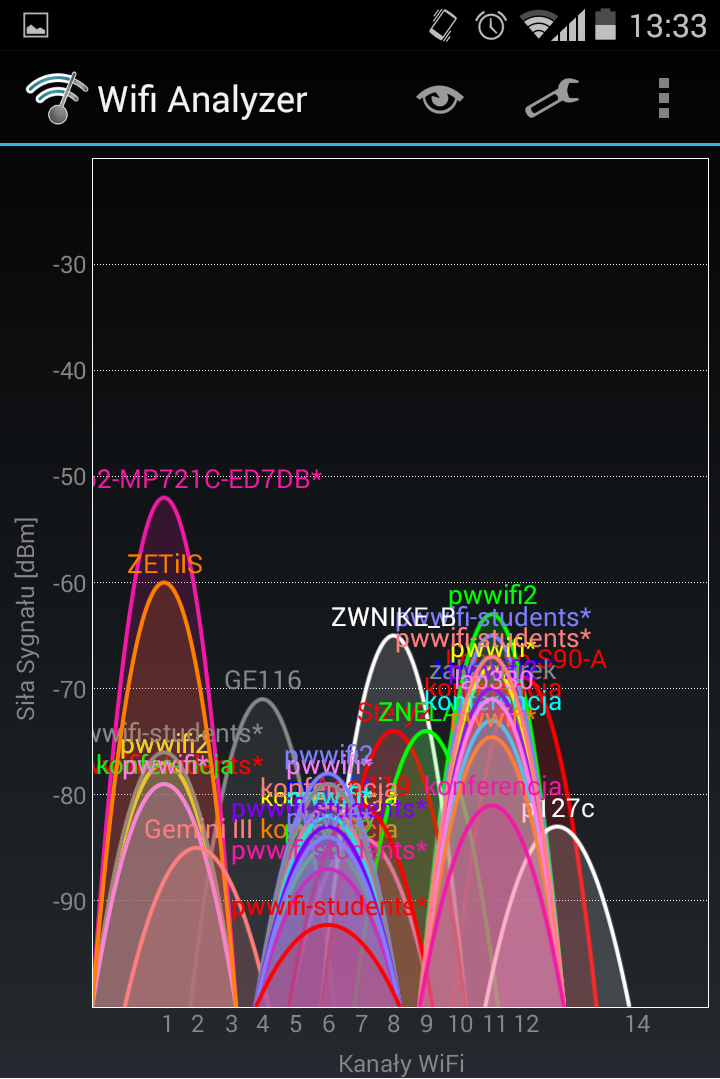
\includegraphics[width=0.5\textwidth]{analyzer.png}
  \caption{Wyniki programu Wifi-Analyzer}
  \label{wifi-analyzer}
\end{figure}

Udało nam się również połączyć z siecią ZETiIS za pomocą telefonu z systemem Android.

\section{Podłącznie interfejsów bezprzewodowych}

\subsection{Kreacja interfejsu wlan0}

Do stworzenia interefejsu bezprzewodowego na maszynie k5 posłużyliśmy się skryptem 
\begin{verbatim}
 k5% sterowniki -w
\end{verbatim}
Załadowaliśmy sterowniki karty 
\begin{verbatim}
 k5% sudo kldload if_iwn
 k5% sudo kldload wlan_amrr
\end{verbatim}
Następnie wykreowaliśmy interfejs wirtualny
\begin{verbatim}
 k5% wlan=$(sudo ifconfig wlan create wlandev iwn0)
 k5% sudo ifconfig $wlan country PL
 k5% sudo ifconfig $wlan up
\end{verbatim}
W efekcie otrzymaliśmy podniesiony interfejs \verb+wlan0+, który automatycznie podłączył się do sieci \verb+pwwifi+.
\begin{verbatim}
 k5% ifconfig $wlan
wlan0: flags=8843<UP,BROADCAST,RUNNING,SIMPLEX,MULTICAST> metric 0 mtu 1500
ether 00:24:d7:53:02:84
media: IEEE 802.11 Wireless Ethernet OFDM/36Mbps mode 11ng
status: associated
ssid pwwifi channel 11 (2462 MHz 11g ht/20) bssid 00:24:14:31:2f:b0
regdomain ETSI country PL authmode OPEN privacy OFF txpower 30
bmiss 10 scanvalid 60 bgscan bgscanintvl 300 bgscanidle 250
roam:rssi 7 roam:rate 64 protmode CTS ampdulimit 64k ampdudensity 8
-amsdutx amsdurx shortgi wme bintval 102
\end{verbatim}


\subsection{Połącznie z siecią pwwifi-students}

\subsection{Połącznie z siecią ZETiIS}

\section{Połącznie równy z równym}

\section{Sieć bluetooth} 

\end{document}
